\section{Fiscal Coverage Retraining Cuts False Acceptance Without Raising True Success}\label{sec:coverage}

\begin{figure*}[tbp]
\centering
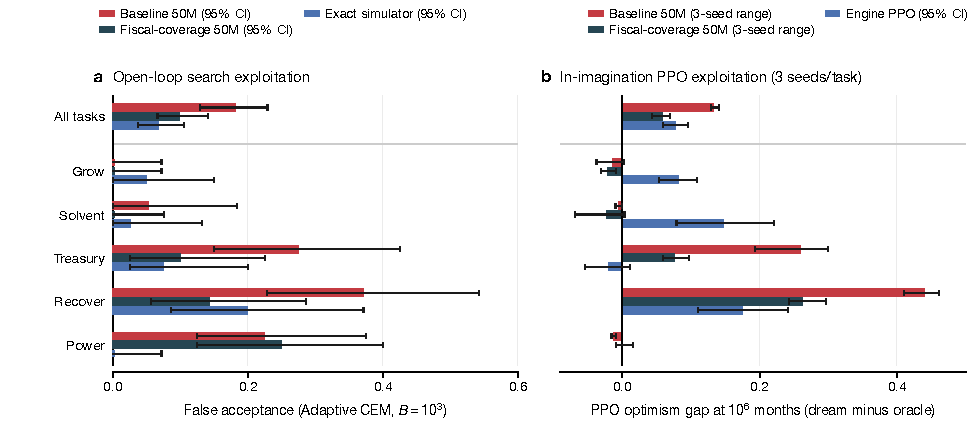
\includegraphics[width=\textwidth]{figures/fig_coverage.pdf}
\caption{\textbf{Retraining on under-covered fiscal regimes cuts exploitation sharply on fiscal and recovery tasks without improving ground-truth pass rates.} Core benchmark (\HeldOutFamilies{} cities) comparing the primary \SizeM{} model (crimson) against an identical model retrained on \CovUnionTransitions{} fiscal-coverage transitions (deep petrol) and the exact-simulator reference (steel blue; error bars in \textbf{a} denote \CILevel{} per cent cluster-bootstrap intervals). \textbf{a}, Adaptive CEM false acceptance at $B ={}$\Bp{3} (\CovSdAdExcessDiff{} \ci{\CovSdAdExcessDiffCI} vs.\ three-seed baseline mean). \textbf{b}, PPO optimism gap after \RlMonths{} steps (\CovRlSeeds{} seeds/cell, seed means and min-max ranges on world-model policies vs.\ \CILevel{} per cent city-bootstrap interval on engine-trained PPO, steel blue).}
\label{fig:coverage}
\end{figure*}

Inspecting policy instruments on \emph{treasury} and \emph{recover} reveals a sharp fiscal support gap. Engine-optimal plans cut tax rates to at most \CovLowTax{} per cent to accelerate migration before harvesting year-two base growth or post-quake rebuilding. Yet only \CovTrainLowTax{} of active building months in our \TrainTransitions-transition training store occupy this regime, compared with \CovFrontLowTax{} among top plans found by engine search. We expand the training store by forty per cent to \CovUnionTransitions{} verified transitions without touching held-out cities or task bars, combining uniformly sampled fiscal grids (\CovUniformTransitions{} transitions) with task-competent constant budgets under periodic month-one earthquakes (\CovCompetentTransitions{} transitions; Appendix~\ref{app:coverage}). Retraining a single seed of the primary \SizeM{} architecture from scratch for the identical \HpSamplesOs{}-example budget (\CovMeetsBar{} all short-horizon gates) is \CovSeedsSentence{}

Under adaptive CEM at $B ={}$\Bp{3}, coverage retraining cuts pooled excess false acceptance from \CovAdAllMainExcess{} \ci{\CovAdAllMainExcessCI} to \CovAdAllCovExcess{} \ci{\CovAdAllCovExcessCI} (paired reduction \CovAdAllDiffExcess{} \ci{\CovAdAllDiffExcessCI}; Figure~\ref{fig:coverage}a), with matching gains on well-posed instances and under random shooting (Appendix~\ref{app:coverage}). Raw false acceptance drops to \CovAdTreasCovHack{} on \emph{treasury} and \CovAdRecovCovHack{} on \emph{recover}, whereas \emph{power} (governed by discrete grid topology rather than fiscal covariates) stays unchanged. Across \CovRlSeeds{} PPO seeds per task, net pass-rate optimism over engine-trained PPO falls by \CovRlGapDiff{} \ci{\CovRlGapDiffCI} overall, driven by \emph{treasury} and \emph{recover} (Figure~\ref{fig:coverage}b).

Yet ground-truth planning capability does not improve. Oracle pass rates under \Bp{3} adaptive CEM match the primary model (\CovAdAllCovOrAcc{} vs.\ \CovAdAllMainOrAcc{}; difference \CovAdAllDiffOrAcc{} \ci{\CovAdAllDiffOrAccCI}, vs.\ \CovAdAllPerfOrAcc{} reference). \CovFalseRejSentence{} Despite a modest logged-plan ranking gain (\CovDecFidDiff{} \ci{\CovDecFidDiffCI}), better OOD calibration under active search turns false passes into rejections without discovering stronger real-world plans (Appendix~\ref{app:coverage}). Unlike sixfold extended training on the unchanged store (Section~\ref{sec:extended}), fiscal coverage retraining cuts excess at the matched two-epoch budget without zero-acceptance collapse (\CovAdAllCovFalseRej{} false rejection).
